\section{Advection}
Following \textcite{schaer2002}, a scalar tracer is transported above the orography by solving the advection equation for a prescribed horizontal wind.  \TODO{what does the test demonstrate?  that the effect of the grid dominates the numerical error}
The wind profile, terrain profile and initial tracer field are shown in Figure~\ref{fig:advection:initial}.

\subsection{Specification}
The domain is \SI{300}{\kilo\meter} wide and \SI{25}{\kilo\meter} high.  The terrain is wave-shaped, specified by the surface height $\surface$ such that
\begin{align}
	\surface(x) &= \cos^2 \left( \frac{\pi x}{\lambda} \right) \surface^\star
%
	\intertext{where}
%
	\surface^\star(x) &= \left\{ \begin{array}{l l}
		h_0 \cos^2 \left( \frac{\pi x}{2a} \right) & \quad \text{if $| x | < a$} \\
		0 & \quad \text{otherwise}
	\end{array} \right.
\end{align}
where $a = \SI{25}{\kilo\meter}$ is the mountain half-width, $h_0 = \SI{3}{\kilo\meter}$ is the maximum mountain height, and $\lambda = \SI{8}{\kilo\meter}$ is the wavelength.  On the SLEVE grid, the large-scale component $\surface_1$, as described in section~\ref{sec:theory:sleve}, is given by
\begin{align}
	\surface_1(x) &= \frac{1}{2}\surface^\star(x)
\end{align}
and $s_1 = \SI{15}{\kilo\meter}$ is the large scale height, and $s_2 = \SI{2.5}{\kilo\meter}$ is the small scale height.  The optimisation of SLEVE by \textcite{leuenberger2010} is not used, so the exponent $n = 1$.

For comparison, the same tests were performed with no orography, such that $\surface = \SI{0}{\kilo\meter}$ everywhere.

The wind is entirely horizontal and is prescribed as
\begin{align}
	u(z) = u_0 \left\{ \begin{array}{l l}
		1 & \quad \text{if $z \geq z_2$} \\
		\sin^2 \left( \frac{\pi}{2} \frac{z - z_1}{z_2 - z_1} \right) & \quad \text{if $z_1 < z < z_2$} \\
		0 & \quad \text{otherwise}
	\end{array} \right.	
\end{align}
where $u_0 = \SI{10}{\meter\per\second}$, $z_1 = \SI{4}{\kilo\meter}$ and $z_2 = \SI{5}{\kilo\meter}$.
This results in a constant wind aloft, and zero flow at \SI{4}{\kilo\meter} and below.
A tracer $\varphi$ is positioned upstream above the height of the terrain.  It has the shape
\begin{align}
	\varphi(x, z) &= \varphi_0 \left\{ \begin{array}{l l}
		\cos^2 \left( \frac{\pi r}{2} \right) & \quad \text{if $r \leq 1$} \\
		0 & \quad \text{otherwise}
	\end{array} \right.
%
\intertext{having radius $r$ given by}
%
	r &= \sqrt{
		\left( \frac{x - x_0}{A_x} \right)^2 + 
		\left( \frac{z - z_0}{A_z} \right)^2
	}
\end{align}
where $A_x = \SI{25}{\kilo\meter}$, $A_z = \SI{3}{\kilo\meter}$ are the horizontal and vertical half-widths respectively, and $\varphi_0 = 1$ is the maximum magnitude of the anomaly.  At $t = \SI{0}{\second}$, the anomaly is centred at $(x_0, z_0) = (\SI{-50}{\kilo\meter}, \SI{9}{\kilo\meter})$ so that the anomaly is upwind of the mountain and well above the maximum terrain height of \SI{3}{\kilo\meter}.  Analytic solutions can be found by adjusting the anomaly centre such that $x_0 = ut$.

\begin{figure}
	\centerfloat
	\input{advection-initial-plot}
	\caption{Vertical cross section of the two-dimensional advection test showing the horizontal wind profile, surface terrain profile and scalar tracer field at $t = \SI{0}{\second}$ on a $\SI{300}{\kilo\meter} \times \SI{25}{\kilo\meter}$ domain.  Adapted from \textcite{schaer2002}.}
	\label{fig:advection:initial}
\end{figure}

\subsection{Discretisation}
The OpenFOAM solver \shellcmd{scalarTransportFoam} was used to implicitly solve the advection-diffusion equation in flux form
\begin{align}
	\frac{\partial \varphi}{\partial t} + \del \cdot \left( \vect{u} \varphi \right) - \laplace \left( \diffusioncoeff \varphi \right) = 0 \label{eq:advection:continuous}
\end{align}
Diffusion was turned off by setting the diffusion coefficient $\diffusioncoeff$ to be zero.

The time derivative ($\partial \varphi / \partial t$) is solved implicitly using a backward-in-time, second order accurate scheme defined as \autocite{openfoam-progguide}
\begin{align}
	\frac{\partial}{\partial t} \int_V \varphi \diff V = \frac{
		3 \left( \varphi V \right)^{(n)} - 
		4 \left( \varphi V \right)^{(n-1)} + 
		\left( \varphi V \right)^{(n-2)}
	}{2 \Delta t}
\end{align}

Spatial discretisation follows the finite volume method described in section~\ref{sec:theory:fv}.
Two spatial interpolations were tested.  First, the van Leer scheme which blends two schemes to maximise boundedness and accuracy.  It combines a centred difference scheme that is second-order accurate and unbounded with an upwind scheme that is first-order accurate and bounded.  The interpolated value $\varphi_F$ is calculated as a weighted average of the interpolated values from the two schemes, $\varphi_{F,\mathrm{upwind}}$ and $\varphi_{F,\mathrm{centred}}$, such that
\begin{align}
	\varphi_F &= \left( 1 - \gamma \right) \varphi_{F,\mathrm{upwind}} + \gamma \varphi_{F,\mathrm{centred}}
\end{align}
The van Leer scheme defines the blending coefficient $\gamma$ as a function of the ratio $r$ between the upwind and local gradient of $\varphi$.  The blending coefficient is specified as \autocite{leveque2002}
\begin{align}
\gamma(r) &= \frac{r + |r|}{1 + |r|}
%
\intertext{and the gradient ratio is specified by \textcite{weller2012} as}
%
	r &= \frac{2 \left( \vect{x_d} - \vect{x_u} \right) \cdot \del_u \phi}{\varphi_d - \varphi_u} - 1
\end{align}
where $\vect{x}$ is the position vector of the cell centre and subscripts $u$ and $d$ denote upwind and downwind cells respectively.

\TODO{Second, a TVD limited version of upwind-biased cubic scheme...  I might not have time to discuss this, but it does offer a modest improvement at the expense of increased computation}

The domain is discretised onto a grid having $300 \times 50$ cells such that $\Delta x = \SI{1}{\kilo\meter}$ and $\Delta \trans{z} = \SI{500}{\meter}$.  Unlike \textcite{schaer2002} which used periodic lateral boundaries, we use zero gradient boundary conditions for all boundaries.
Tests are integrated forward in time for \SI{10000}{\second} with a timestep $\Delta t = \SI{25}{\second}$.  \TODOsidenote{we never looked at courant numbers, but Schaer talks about horiz/vertical Co numbers}

\subsection{Results}
\begin{figure}
	\captionsetup[subfigure]{position=b}
	\centering
	\subcaptionbox{BTF \label{fig:advection:vanLeer:btf}}[0.49\textwidth]{\input{advection-btf-schaerCos-vanLeer-contour-plot}}
	\hfill
	\subcaptionbox{BTF \label{fig:advection:schaer:btf}}[0.49\textwidth]{\vspace{0.43in}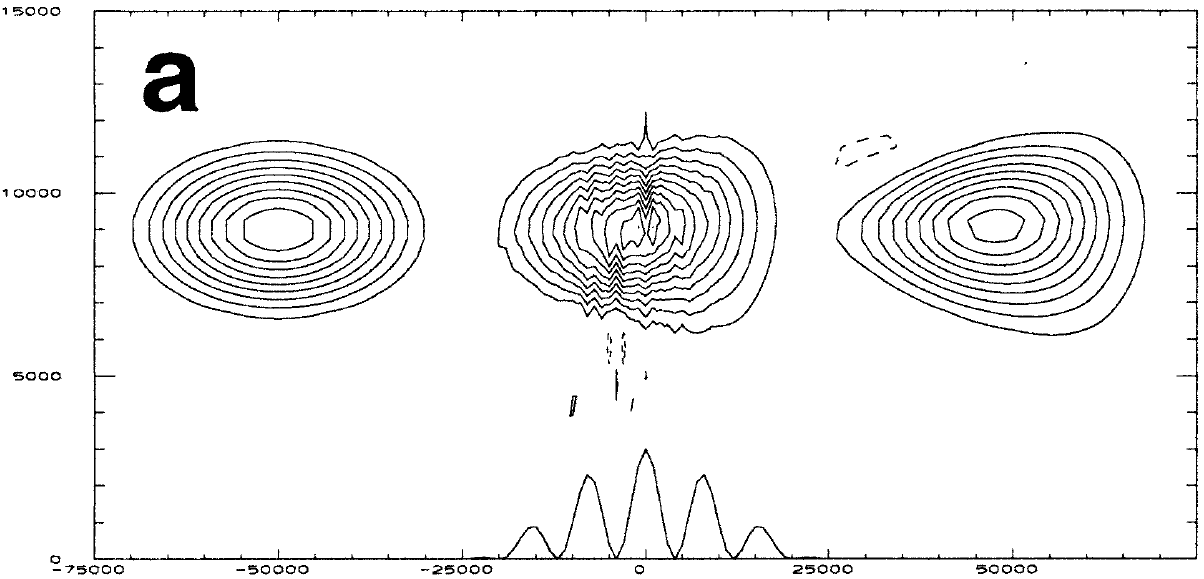
\includegraphics[height=1.2in]{img/schaer-btf-centred.png}}
\\
	\subcaptionbox{SLEVE \label{fig:advection:vanLeer:sleve}}[0.49\textwidth]{\input{advection-sleve-schaerCos-vanLeer-contour-plot}}
	\hfill
	\subcaptionbox{SLEVE \label{fig:advection:schaer:sleve}}[0.49\textwidth]{\vspace{0.43in}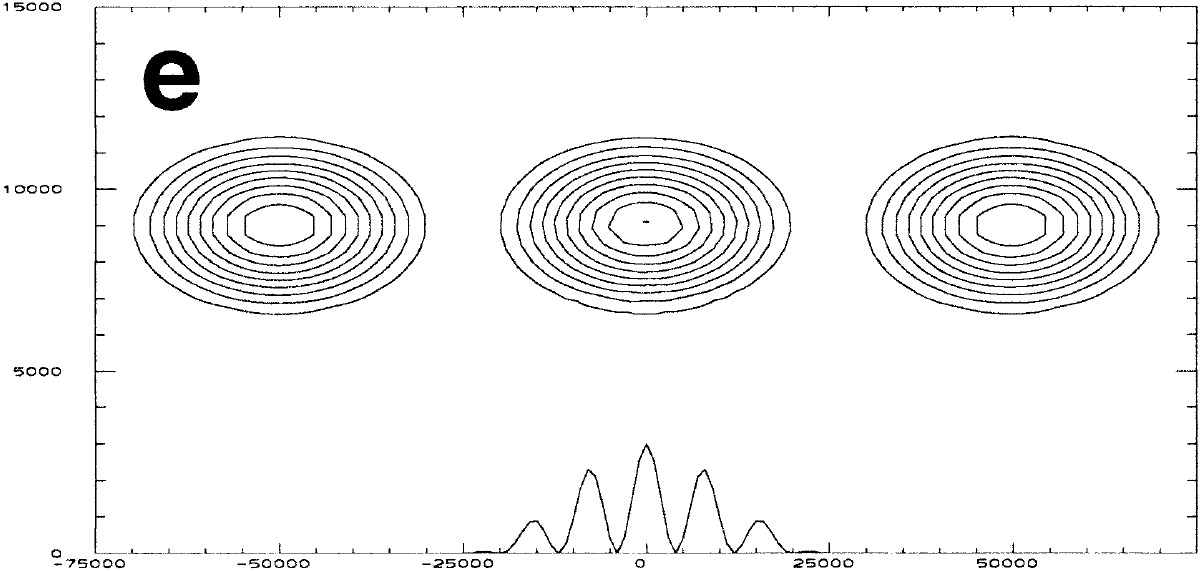
\includegraphics[height=1.2in]{img/schaer-sleve-centred.png}}
\\
	\subcaptionbox{Cut cell \label{fig:advection:vanLeer:cutCell}}[0.49\textwidth]{\input{advection-snapCol-schaerCos-vanLeer-contour-plot}}
	\hfill
	\subcaptionbox{Analytic solution on a regular grid}[0.49\textwidth]{\input{advection-noOrography-analytic-contour-plot}}
%
	\caption{\TODO{van Leer advection compared with schaer -- centred scheme.  Contour intervals every 0.1}}
	\label{fig:advection:vanLeer}
\end{figure}

Results of advection using the van Leer scheme are presented in Figure~\ref{fig:advection:vanLeer}.  On the BTF grid, the tracer suffers from distortion over the mountain and some artefacts just above the mountain remain as the tracer moves over it.  Compared with the results from \textcite{schaer2002}, the tracer retains more of its shape but suffers from far more numerical diffusion by the end of the simulation, as evidenced by the missing contours in the tracer centre.  \TODO{would it be worth looking at variance at t=10000s to quantify the diffusion?}

Results on the SLEVE grid are much closer to the analytic solution on a regular grid.  The tracer retains its shape throughout the simulation and does not suffer from any noticeable distortion.  However, the widening contours indicate some numerical diffusion is still present which, again, was not found in the results of \textcite{schaer2002}.

Since the cut cell grid is entirely regular away from the surface, it is unsurprising that the results are the same as advection on a regular grid (not shown).  This result agrees with that found by \textcite{good2013}.

\TODO{we could try plotting diffs as done by schaer2002, too}

\TODO{now discuss tvdLimitedCubicUpwindCPCFit}
\TODO{tvdLimitedCubicUpwindCPCFit slightly better than vanLeer, but much more computationally expensive}

Error norms were calculated at $t = \SI{10000}{\second}$ by comparing with the analytic solution.  The $\ell^2$ error norm is defined as
\begin{align}
\ell^2 = \sqrt{\frac{\sum \left( \varphi - \varphi_T \right)^2 \cdot V}{\sum V}}
\end{align}
where $\varphi$ is the numerical tracer value, $\varphi_T$ is the analytical value and $V$ is the cell volume.  Because the test is two dimensional, the cell volume is equivalent to the cell area.  The resulting errors are summarised in table~\ref{tab:advection:errors}.  \TODO{what do they tell us?}

\begin{table}
\centering
\begin{tabular}{ r @{\hspace{2em}} l l}
\toprule
		&	van Leer	& Cubic upwind \\ \midrule
BTF		& \input{openfoam/cases/advection/btf/schaerCos/vanLeer/l2error.txt}		& \TODO{0} \\
SLEVE		& \input{openfoam/cases/advection/sleve/schaerCos/vanLeer/l2error.txt}		& \TODO{0} \\
Cut cell	& \input{openfoam/cases/advection/snapCol/schaerCos/vanLeer/l2error.txt}	& \TODO{0} \\ \bottomrule
\end{tabular}

\caption{$\ell^2$ error norms for the advection test at $t = \SI{10000}{\second}$}
\label{tab:advection:errors}
\end{table}

